\documentclass[a4paper,12pt]{article}

% Packages
\usepackage[utf8]{inputenc} % UTF-8 encoding
\usepackage{amsmath} % Math symbols and environments
\usepackage{graphicx} % Include graphics
\usepackage{hyperref} % Hyperlinks in document
\usepackage{cleveref} % Better referencing
\usepackage{geometry} % Page layout
\usepackage{caption} % Custom captions for figures

% Page layout
\geometry{margin=1in} % 1 inch margins

% Title and Author
\title{GDSFactory Libraries Study Notes}
\author{Your Name}
\date{\today}

\begin{document}

\maketitle

\tableofcontents % Table of contents

\section{Introduction}

GDSFactory is a Python library for designing and simulating photonic circuits. This document serves as a study guide for understanding the key components and functionalities provided by the GDSFactory libraries.

\section{Basic Concepts}

\textbf{Notes about the simulating method used in Pernice and Schuck groups}

An important figure about the method used in this thesis is shown in \cref{fig:sim_methods}.

\begin{figure}[h]
  \centering
  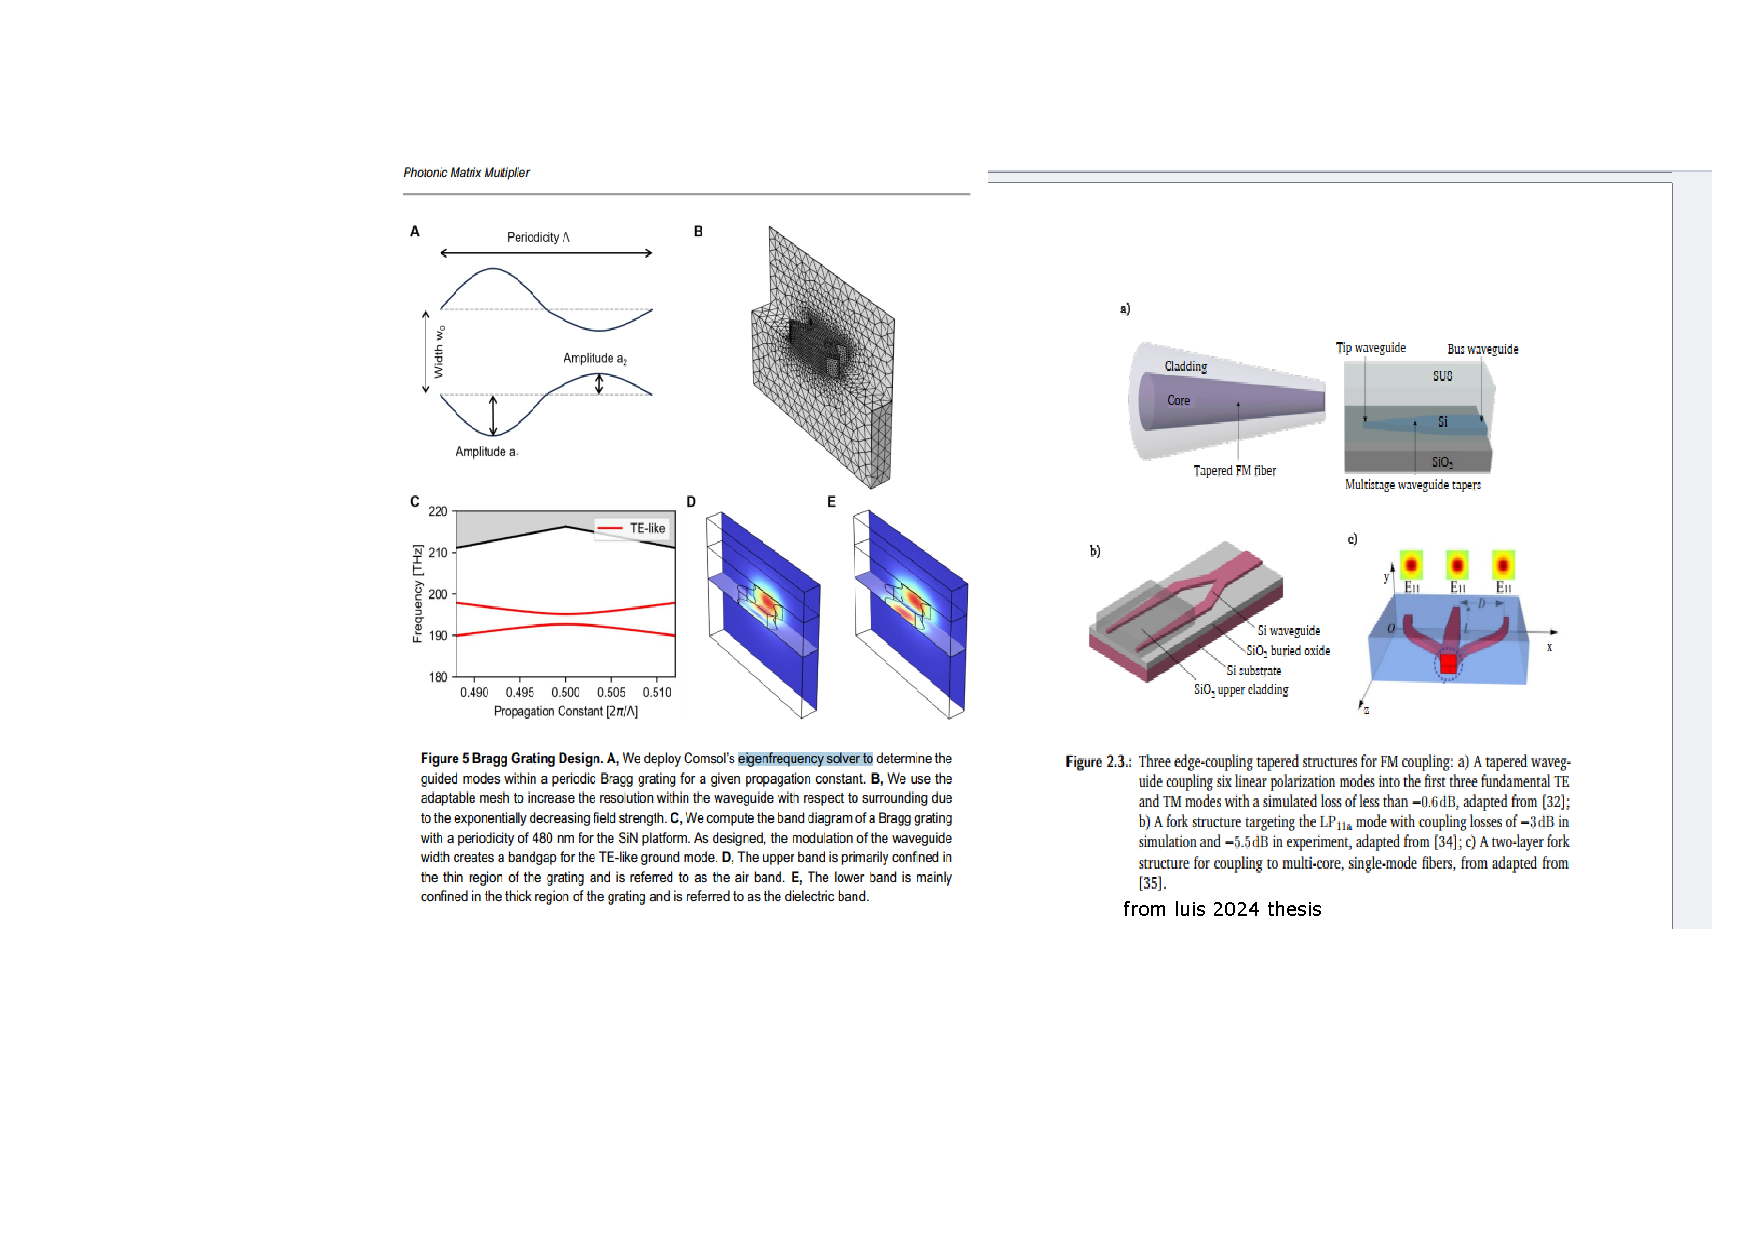
\includegraphics[width=0.6\textwidth]{figs/sim_methods.pdf} % Include your figure here
  \caption{Example of simulation methods from thesis print 2024.}
  \label{fig:sim_methods}
\end{figure}


\begin{figure}[h]
  \centering
  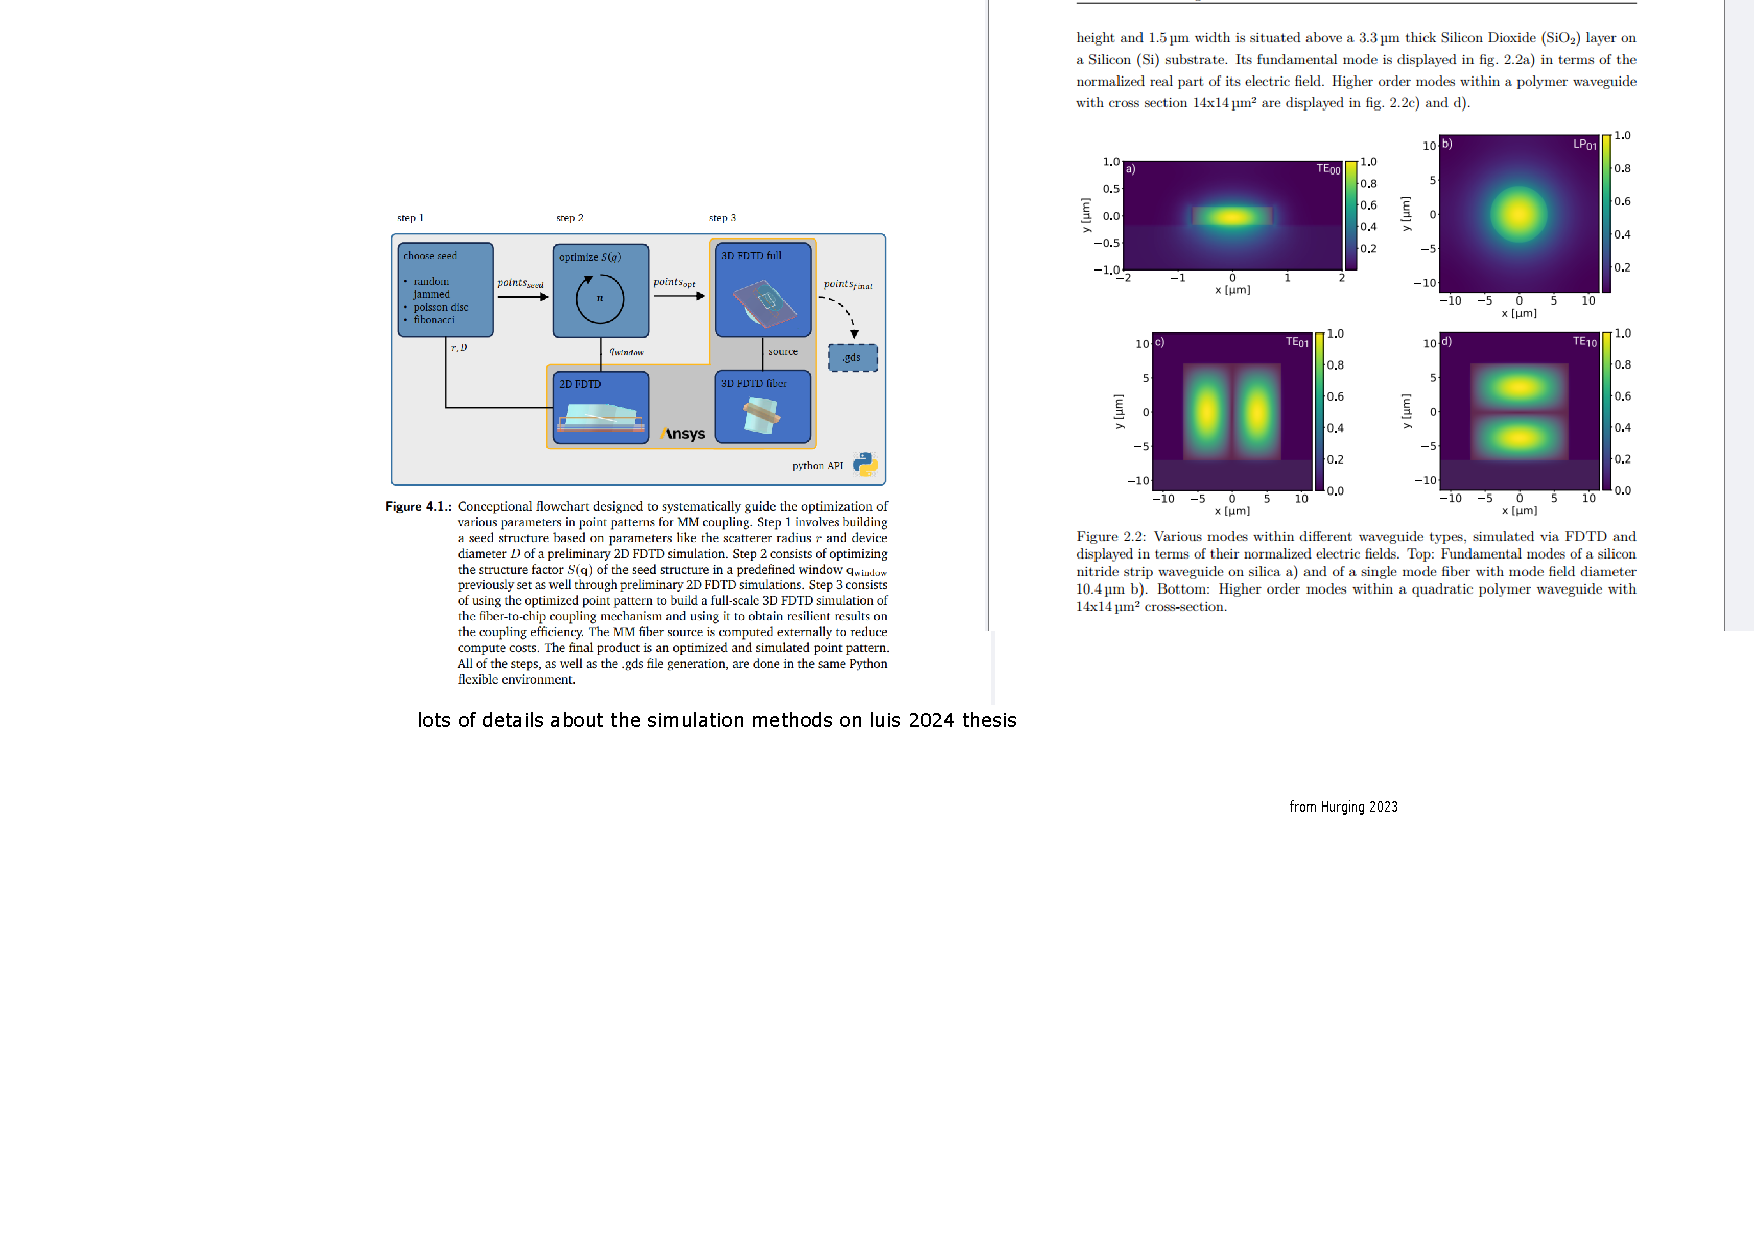
\includegraphics[width=0.6\textwidth]{figs/sim_1.pdf} % Include your figure here
  \caption{Example of simulation methods from thesis Heuging  2023.}
  \label{sim_1}
\end{figure}

\begin{figure}[h]
  \centering
  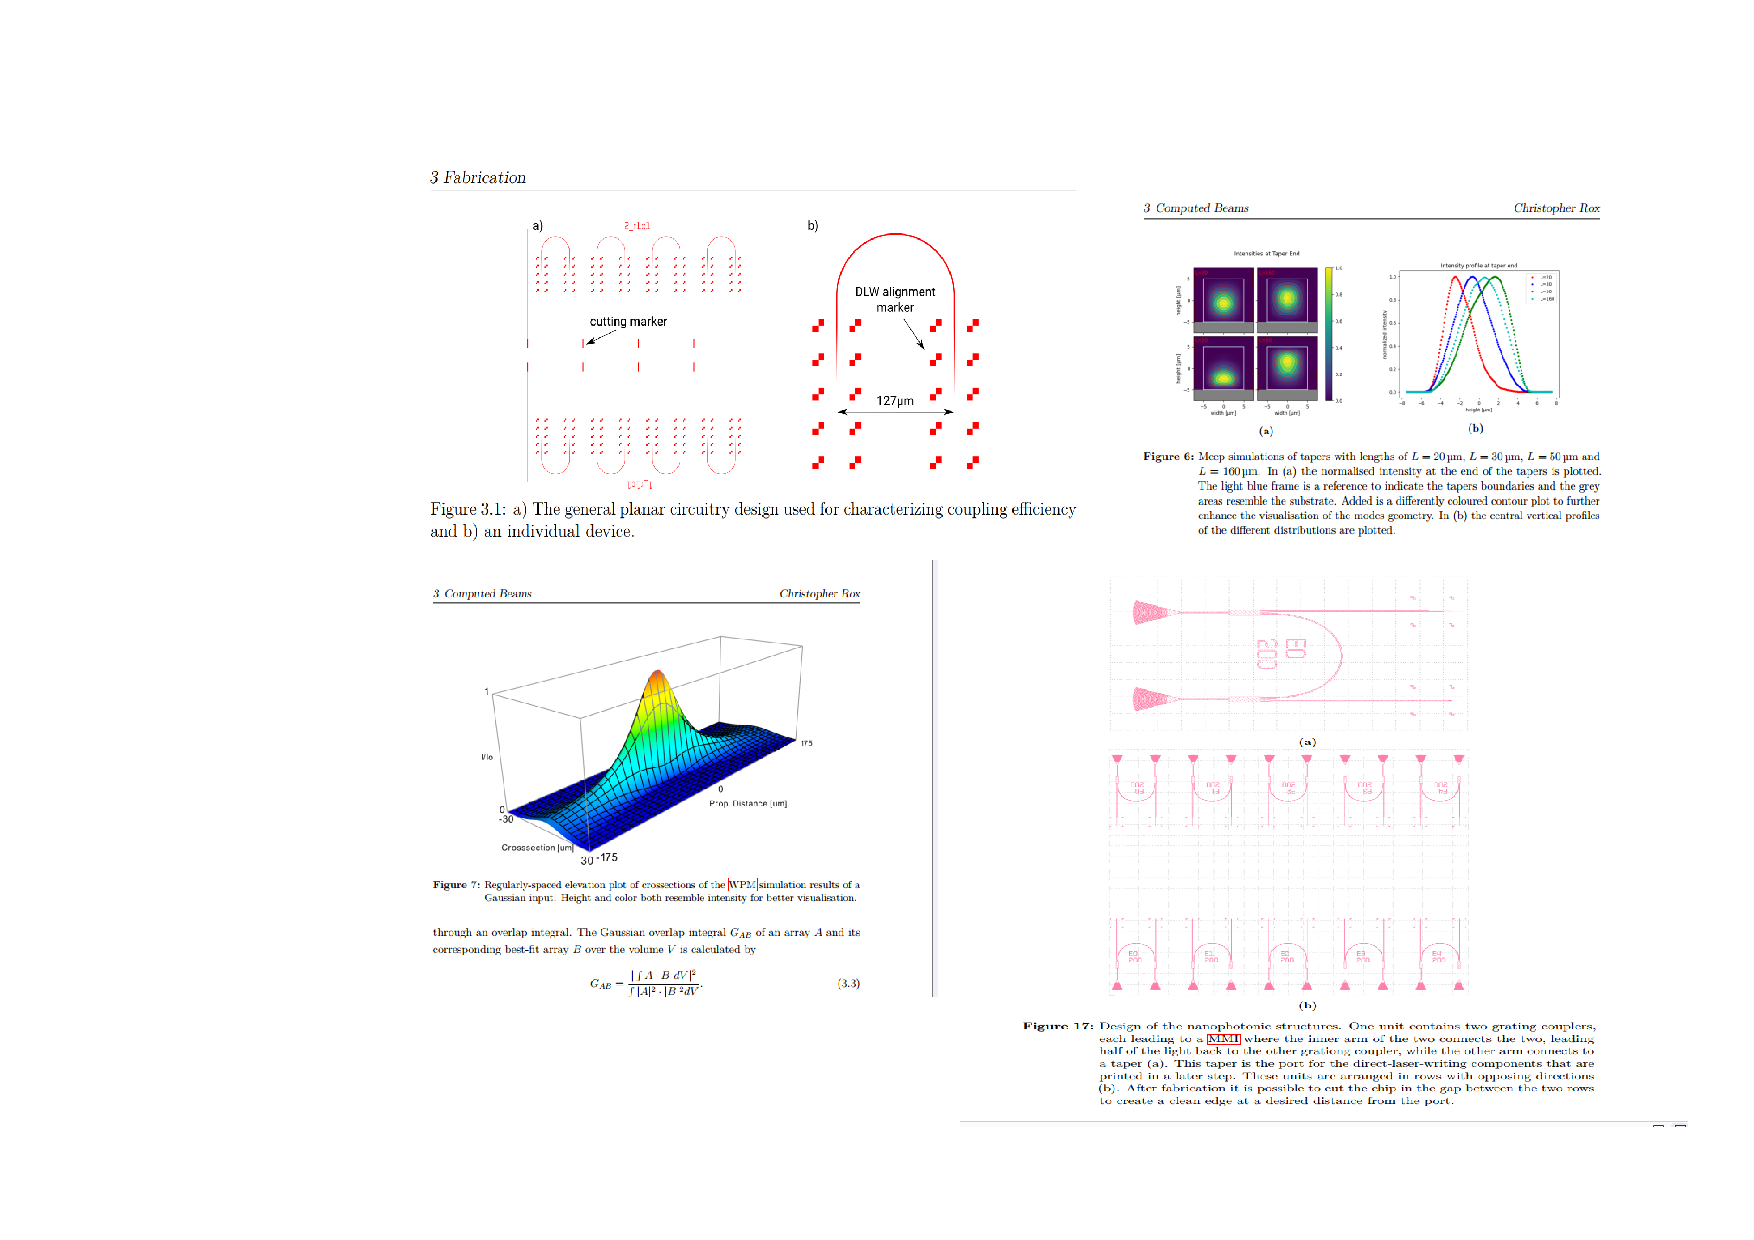
\includegraphics[width=0.6\textwidth]{figs/sim_2.pdf} % Include your figure here
  \caption{Example of simulation methods from thesis Heuging  2023.}
  \label{sim_1}
\end{figure}


\begin{figure}[h]
  \centering
  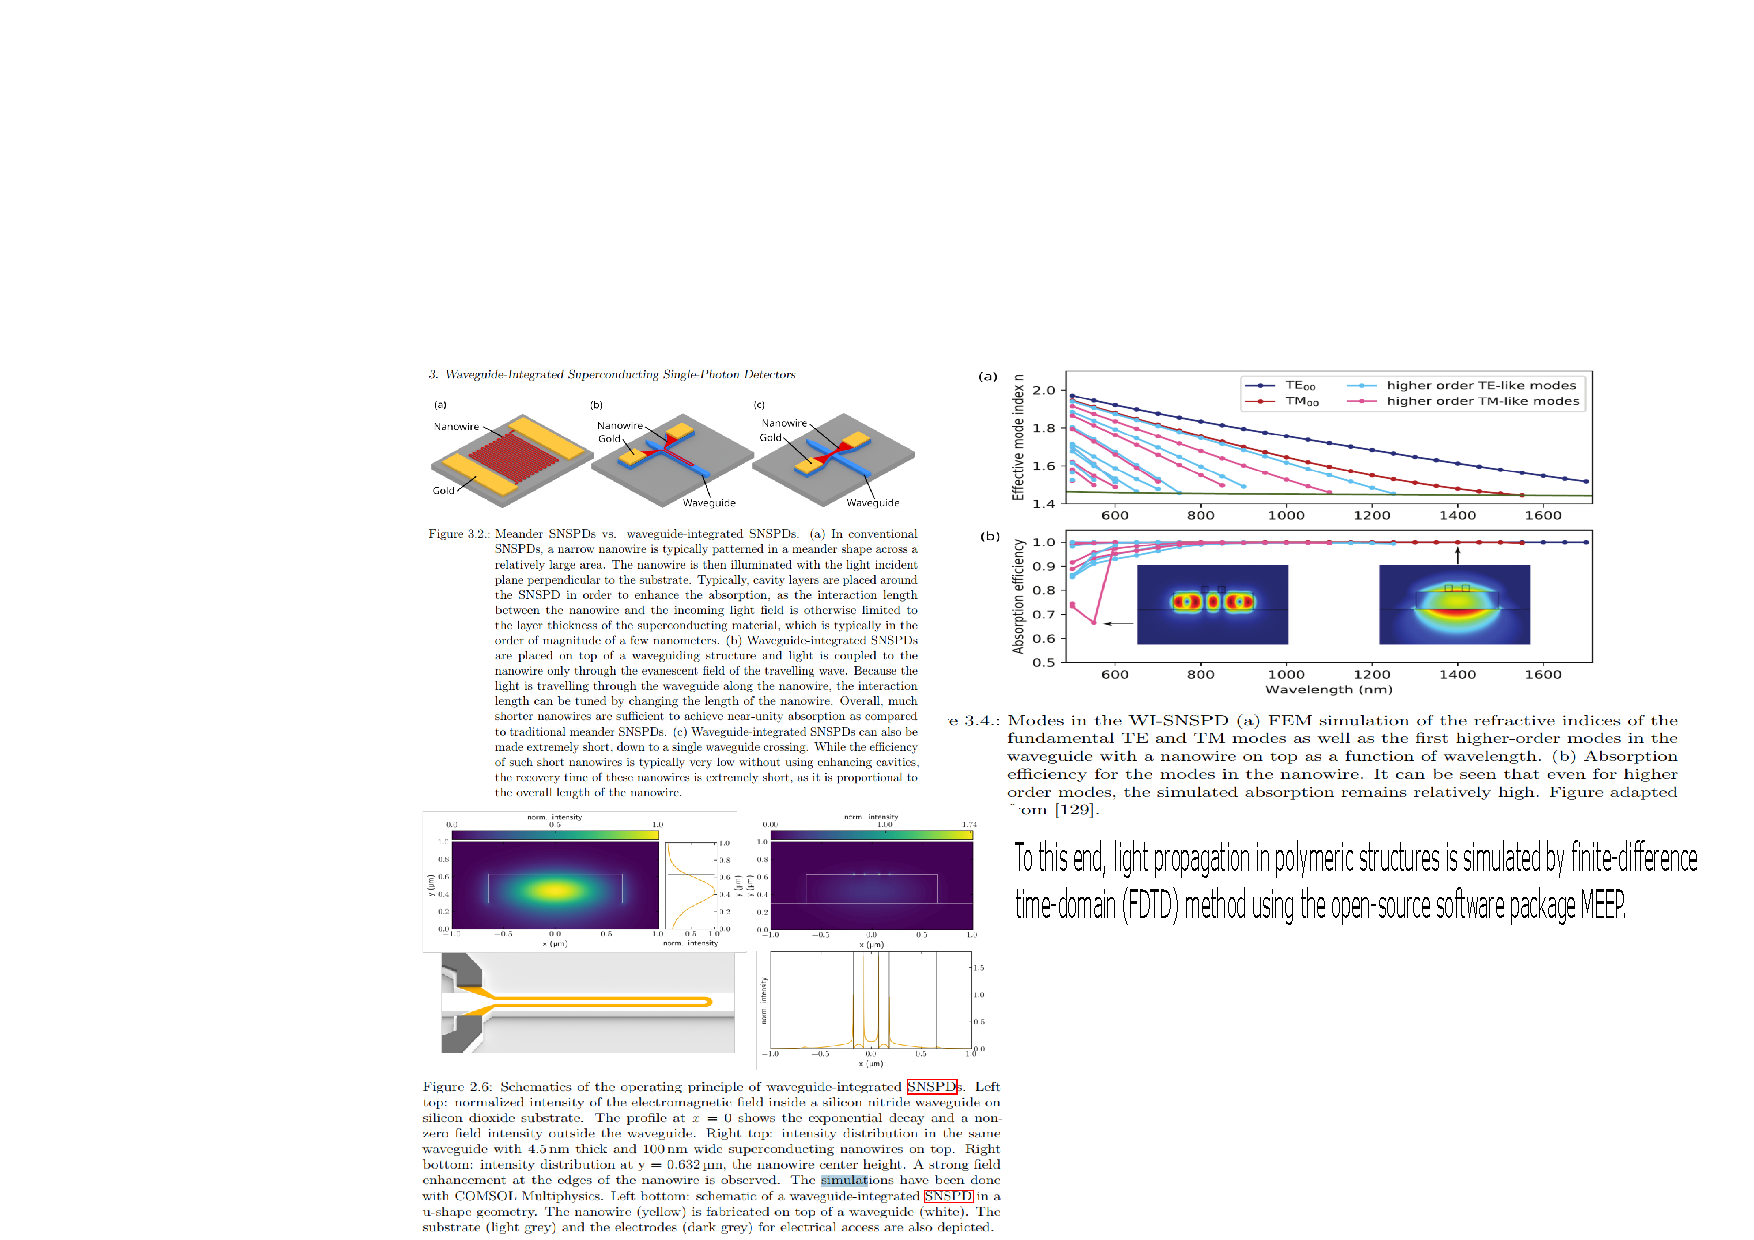
\includegraphics[width=0.6\textwidth]{figs/sim_3.pdf} % Include your figure here
  \caption{Example of simulation methods from thesis Heuging  2023.}
  \label{sim_1}
\end{figure}









\section{Conclusion}

This document provides a basic overview of studying GDSFactory libraries. Further sections can be added to explore more advanced features and functionalities.

\end{document}

